\subsection{LSTM}

Next, we worked on Long Short-Term Memory (LSTM) networks, a type of Recurrent Neural Network, to classify toxic comments in online platforms. LSTMs are adept at processing sequential data, making them ideal for natural language processing tasks where understanding context and dependencies in text is crucial. LSTMs stand out for their ability to maintain memory of previous inputs through internal states, enabling them to capture temporal dependencies in sequential data like text. This makes them particularly well-suited for text classification tasks.

\subsubsection{Preprocessing and Data Preparation}
\begin{itemize}
    \item The dataset, comprising text comments and toxicity labels, undergoes preprocessing using Keras’s \texttt{Tokenizer}. This tokenizer focuses on the top 20,000 most frequent words (\texttt{max\_features}) to balance relevance and computational efficiency.
    \item Tokenized text is converted into sequences of uniform length (\texttt{maxlen} of 200 tokens) to ensure consistency in input size for the LSTM model.
\end{itemize}

\subsubsection{Model Architecture and Parameters}
\begin{itemize}
    \item \textbf{Architecture}: The model features an embedding layer, an LSTM layer with 20 units, a global max pooling layer, and dense layers with dropout (0.1 rate) for regularization. The architecture is designed to balance learning capability with computational efficiency.
    \item \textbf{Embedding Layer}: Converts words into 128-dimensional vectors, capturing semantic relationships in a computationally manageable space.
    \item \textbf{LSTM Layer}: The 20-unit layer is tailored to process sequential data effectively, balancing complexity and learning capacity.
    \item \textbf{Dense Layers and Activation}: Includes `relu` activation for intermediate processing and `sigmoid` for the final output, appropriate for binary classification in multi-label contexts.
    \item \textbf{Optimizer and Loss Function}: Utilizes the Adam optimizer for adaptive learning and binary cross-entropy loss, suitable for multi-label classification tasks.
    \item \textbf{Input Parameters}: Limits vocabulary to the top 20,000 words and pads sequences to a maximum length of 300 tokens, ensuring relevance and uniform input size.
\end{itemize}


\subsubsection{Training and Evaluation}
The model is trained for 5 epochs with a batch size of 32, a setup that balances training speed and model performance, aiming to minimize overfitting while ensuring adequate learning. We tuned parameters such as lstm layer units, dense layer units and \texttt{max\_len}.

We selected the following values for these parameters:
\begin{itemize}
    \item LSTM layer units: 20
    \item Dense layer units: 70
    \item Max Length of tokens: 300
\end{itemize}

The graphs associated to our tuning improvement can be found at fig \ref{fig:lstm_parameter_tuning}

\begin{figure}%
    \centering
    \subfloat[\centering LSTM layer units for AUC vs labels]{{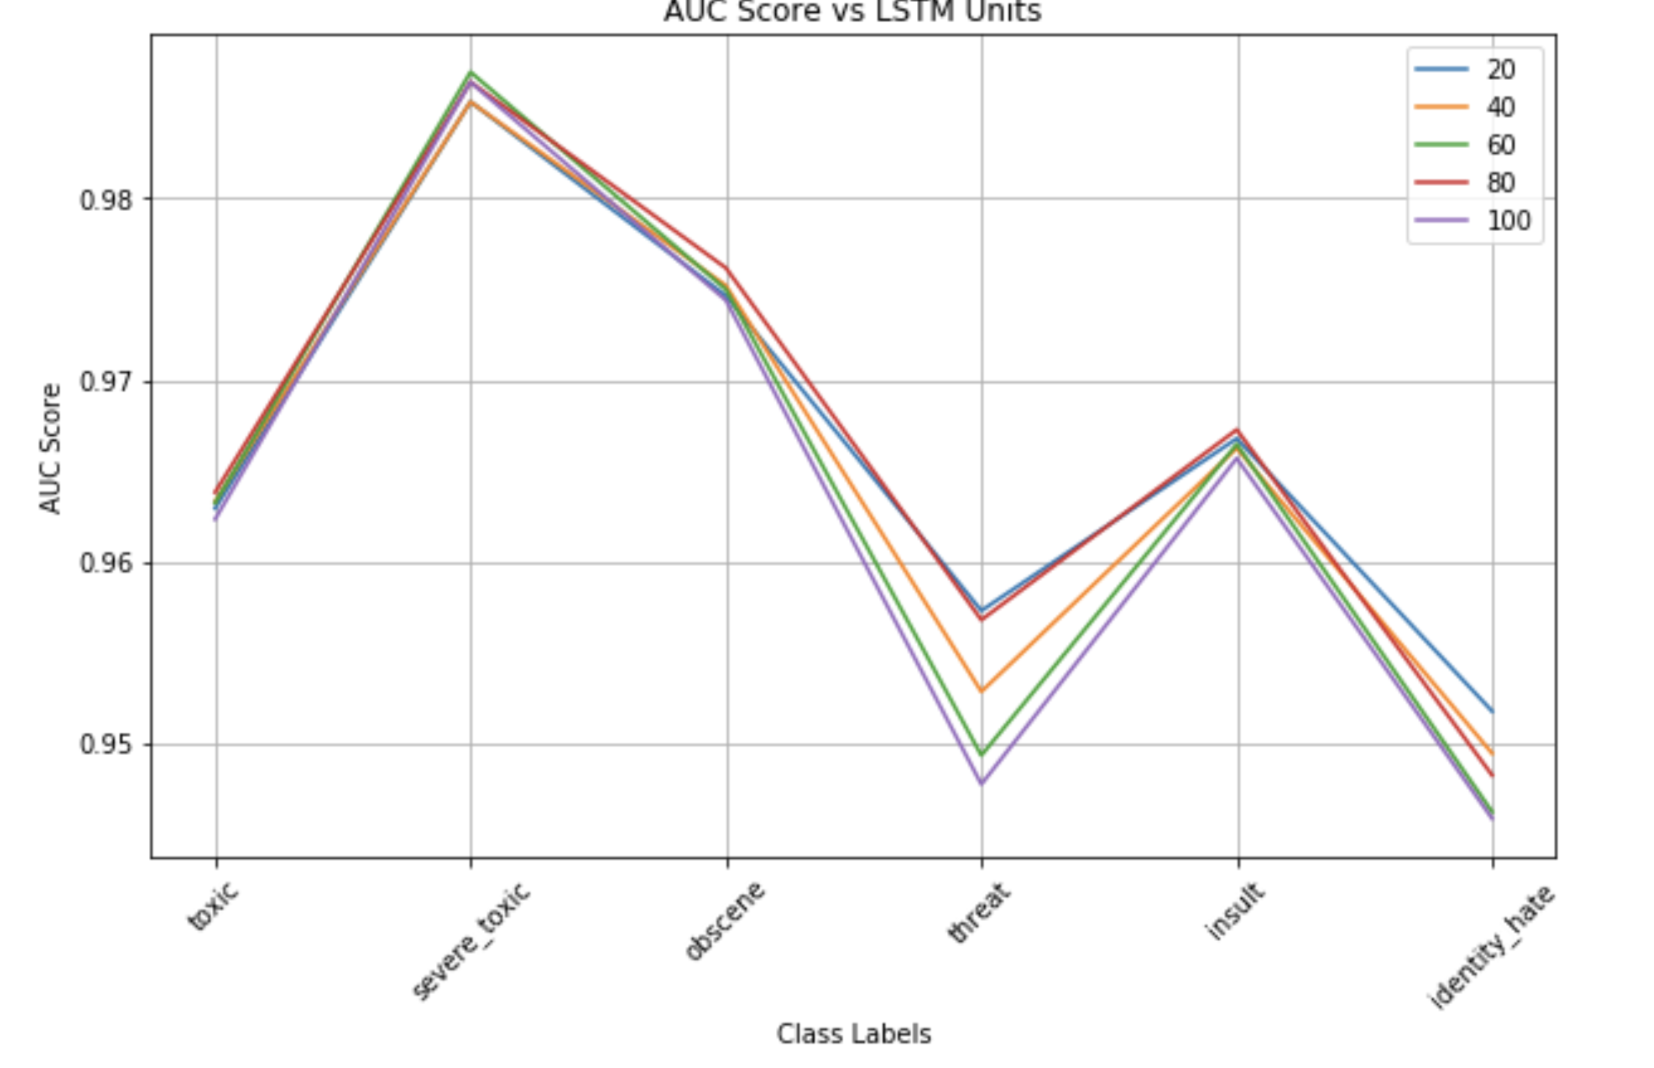
\includegraphics[scale=0.25]{images/graphs/lstm_units.png} }}%
    \qquad
    \subfloat[\centering Dense layer units for AUC vs labels]{{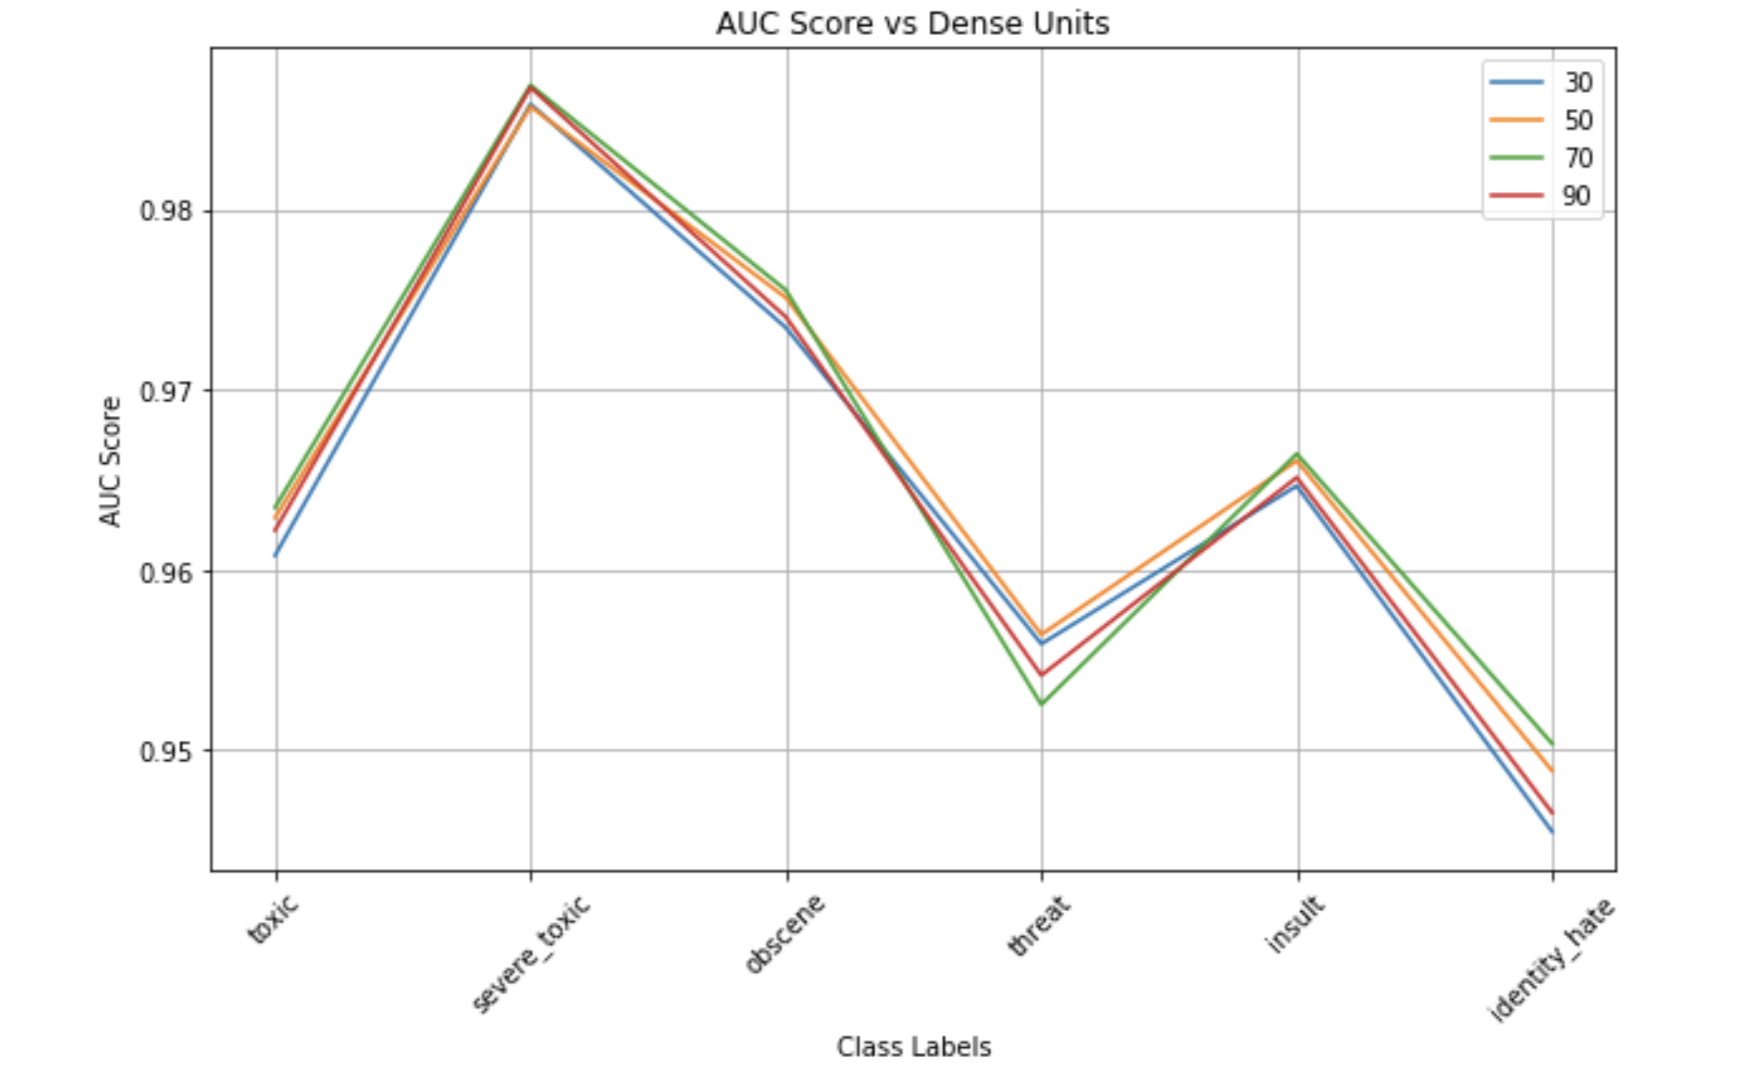
\includegraphics[scale=0.25]{images/graphs/LSTM_DenseUnits.png} }}%
    \qquad
    \subfloat[\centering Max length of tokens for AUC vs labels]{{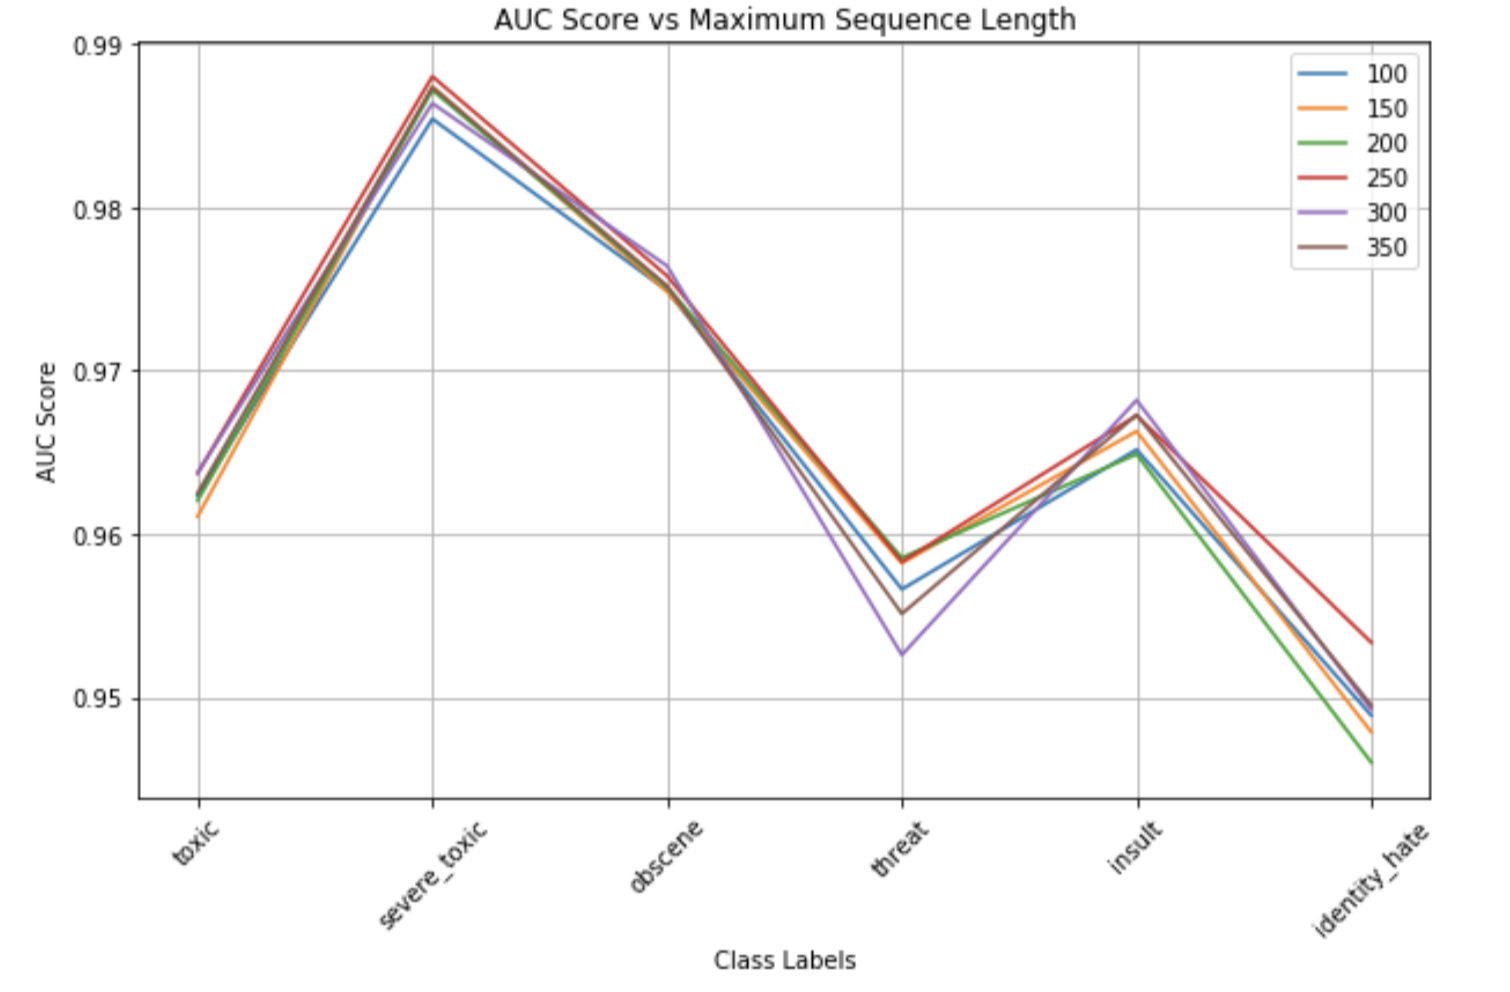
\includegraphics[scale=0.25]{images/graphs/LSTM_MaxLength.png} }}%
    \caption{Dataset Analysis and Visualization}%
    \label{fig:lstm_parameter_tuning}
\end{figure}

The results of test data evaluation can be found at table \ref{tab:model_metrics_lstm}.

\begin{table}[h]
\centering
\begin{tabular}{|c|c|c|c|c|c|}
\hline
 & Test Accuracy (\%) & AUC Score (\%) & F1 Score (\%) & Precision (\%) & Recall (\%) \\
\hline
toxic & 94.16 & 95.80 & 94.53 & 94.95 & 93.16 \\
severe\_toxic & 99.27 & 98.57 & 99.27 & 99.27 & 99.27 \\
obscene & 96.05 & 97.11 & 96.16 & 96.31 & 96.05 \\
threat & 99.68 & 98.16 & 99.60 & 99.58 & 99.68 \\
insult & 96.24 & 96.60 & 96.17 & 96.10 & 96.24 \\
identity\_hate & 99.09 & 97.25 & 98.92 & 98.91 & 99.09 \\
\hline
\textbf{Weighted Avg.} & \textbf{95.58} & \textbf{96.50} & \textbf{95.74} & \textbf{95.94} & \textbf{95.16} \\
\hline
\end{tabular}
\caption{Model Evaluation Metrics for LSTM}
\label{tab:model_metrics_lstm}
\end{table}



\subsubsection{Conclusion}
The LSTM model, with its strategically chosen parameters, presents a robust approach for classifying toxic comments. Its proficiency in handling sequential text data makes it a valuable tool in this domain. Future enhancements might include further parameter optimization, exploring additional feature engineering techniques, or investigating alternative sequence model architectures for improved performance.
